\chapter{Implementation}
\label{sec:implementation}

% Hier greift man einige wenige, interessante Gesichtspunkte der Implementierung
% heraus. Das Kapitel darf nicht mit Dokumentation oder gar Programmkommentaren
% verwechselt werden. Es kann vorkommen, daß sehr viele Gesichtspunkte
% aufgegriffen werden müssen, ist aber nicht sehr häufig. Zweck dieses Kapitels
% ist einerseits, glaubhaft zu machen, daß man es bei der Arbeit nicht mit einem
% "Papiertiger" sondern einem real existierenden System zu tun hat. Es ist
% sicherlich auch ein sehr wichtiger Text für jemanden, der die Arbeit später
% fortsetzt. Der dritte Gesichtspunkt dabei ist, einem Leser einen etwas
% tieferen Einblick in die Technik zu geben, mit der man sich hier beschäftigt.
% Schöne Bespiele sind "War Stories", also Dinge mit denen man besonders zu
% kämpfen hatte, oder eine konkrete, beispielhafte Verfeinerung einer der in
% Kapitel 3 vorgestellten Ideen. Auch hier gilt, mehr als 20 Seiten liest
% keiner, aber das ist hierbei nicht so schlimm, weil man die Lektüre ja einfach
% abbrechen kann, ohne den Faden zu verlieren. Vollständige Quellprogramme haben
% in einer Arbeit nichts zu suchen, auch nicht im Anhang, sondern gehören auf
% Rechner, auf denen man sie sich ansehen kann.

In the following section, I will explain some technical implementation details.
In particular, I want to highlight some of the implementation details of
components explained in chapter~\ref{sec:design}. First, I will refer to Linux,
which I use as the host kernel in the system. A special configuration was used
because I will make it run in parallel to the TEE kernel. Next, in
section~\ref{sec:implementation:teeKernel}, I will introduce phipsboot, which I
use as the TEE kernel, along with the modification I introduced to adapt it to
my use case. Another component I programmed is the Linux kernel module, which I
explain in section~\ref{sec:implementation:kmod}. In the last part of the
implementation chapter, I will explain how I implemented the attack simulations.

% \begin{itemize}
%       \item Chose Linux as Host Kernel, Phipsboot as TEE kernel.
%       \item Implement for Intel Rapter Lake, test system has Intel Core i7 13700k
%       \item I will explain in this chapter:
%             \begin{itemize}
%                   \item How I use the host system, what the kernel module does
%                   \item How does the communication work in detail between TEE kernel
%                         and host OS
%                   \item Why Phipsboot, what modifications?
%                   \item What do the attacks do?
%             \end{itemize}
% \end{itemize}


\section{TEE Kernel: phipsboot}
\label{sec:implementation:teeKernel}

PhipsBoot is a Multiboot 2 compliant kernel mainly written in the memory-safe
programming language Rust, which is designed to be relocatable in the memory. It
depends on a first-stage bootloader\todo{maybe this is not a multi-stage
    bootloader} that brings the system to a state defined in the Multiboot 2
specification. That is, the CPU is in 32-bit mode with segmentation enabled.
After handover, PhipsBoot does all initialization steps to bring the CPU into
64-bit with enabled PEA paging. It initializes the page tables and sets up huge
pages for the initial mapping. PhipsBoot expects to be loaded to a 2 MiB-aligned
address. Its small size, which is less than 2 MiB, allows PhipsBoot to set up
the page table hierarchy using a single page table that maps the kernel.
PhipsBoot uses memory statically reserved for dynamic memory allocation in the
kernel's Elf image. Next to being relocatable, PhipsBoot does not implement more
features but offers a great starting point for implementing the TEE features. \\

The first feature I introduced was modifying page tables. This feature was
lacking because PhipsBoot's purpose does not require the modification of the
page to map, for example, mapping memory that is not contained in its binary.
For this, I modified the page table setup routine and changed the last page
table to be writable instead of read-only. Through observation, I found that not
more than the first 128 entries in the page table are used to map all kernel
memory. For dynamic mapping, I, therefore, reserved the last 128 entries. This
enabled PhipsBoot to map memory that was not contained in the binary. This
feature is important to implement the shared memory communication path. The
address is communicated to PhipsBoot through the Multiboot 2 memory map. To
access this structure, PhipsBoot needs to be able to map the page containing it.
Moreover, the address in the memory map must be mapped by PhipsBoot to make the
shared memory accessible. Other than the memory owned by the kernel, the memory
intended to be used by the TEE kernel and the host kernel is mapped as
uncacheable. This prevents cache pollution and false positives for allowed
access of a remote core to memory, also used by the TEE.\\

To prepare the environment, the TEE kernel needs to ensure that all memory used
by it is in the exclusive or modified state so that a remote core must trigger
an offocre\todo{Irgendwo mal erklären was ein OFfcore event ist} event when it
tries to access memory owned by the TEE kernel. For this, I implemented a
function that iterates over the page table entries and copies all bytes in
place. This triggers the modified state of the cache line, which leads to
invalidating the cache line in remote cores referencing the same memory item.
The TEE can now detect subsequent access from the remote core through monitoring
performance counters. For this, the TEE writes the respective events to the
configuration MSRs. Once prepared, the TEE sets the IDTR to null, which leads to
triple faulting once an interrupt is delivered to the TEE. The only expected
interrupts in the TEE are NMIs, PMIs, and IPIs from other cores. All other
interrupts are masked by clearing the interrupt flag in the EFLAGS register of
the isolated core. \\

NMIs can be sent by faulty hardware and the interrupt controller if configured
accordingly. Currently, the TEE has no other means of defense against malicious
SMM code. IPIs originate from other cores and can be sent by those at any time.
Because IPIs are routed through the IDT, the same countermeasures as with NMIs
are taken. The invalid setting of the IDTR to NULL results in a triple fault
that ultimately results in a reset of the whole machine. The same defense
strategy is employed upon registering an offshore event triggered through a
read-or-write attempt from a remote core. By defining a threshold for event
occurrence upon which overflow emits a PMI, the TEE can terminate as it wishes.
A useful threshold is 1, which results in a PMI triggered by the first
occurrence of the respective event. For this, we use an event that counts all
occurrences of off-core communication not served by main memory. This works
because all memory is placed in the cache, and only the communication routine is
accessing the uncacheable main memory. \\

\begin{center}
    \begin{figure}
        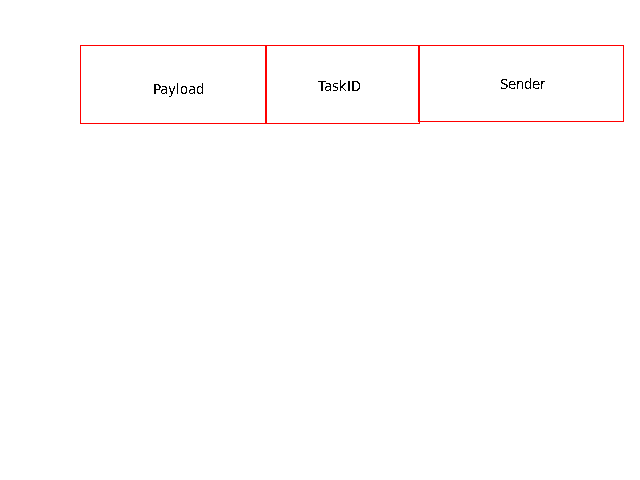
\includegraphics[width=0.8\textwidth]{images/shared_mem_placeholder.png}
        \caption{Shared memory protocol}
        \label{fig:shared-mem}
    \end{figure}
\end{center}
\todo{replace graphic}

I implemented a structure to manage the memory in question to enable
communication through the shared memory channel. Access to the shared memory
follows a simple protocol that splits the memory, as shown in
figure~\ref{fig:shared-mem}. The first byte denotes the sender, the second
denotes the task identifier, and the remaining part is used for a payload that
can be sent along with the other tags. I assume there are only two communication
parties in the current prototype: the TEE kernel and the host kernel. A message
is sent by writing the first byte. To receive a message, the respective party
polls the first byte of the shared memory and waits until the signal is written
by the other party, \\

After initialization, the TEE environment starts a state machine that controls
the execution of tasks. In the first state, the TEE polls the shared memory
until it receives a message containing the command to execute one of the
predefined tasks. Once this message is received, the TEE executes the task as
commended. While the task runs, it can access the shared memory for multiple
reasons. The first reason is that the task can access the payload section of the
memory to receive additional input data from the party outside of the TEE. The
second reason is that the task can prepare an answer to the third-party request.
For this, the task can write to the sender information, the command, and the
payload fields as it wishes. It is the task's responsibility to write to the
shared memory data needed to create a response to the request once it is done.
After the task returns, the TEE creates a report from the performance counters
and sends the result to the third party over the shared memory
channel.\todo{Does it really?} \\

% \begin{itemize}
%     \item MB2 compliant kernel
%     \item expects to be loaded to a memory aligned to 2 MiB
%     \item Relocate able: Can be freely moved in memory -> important as I don't
%           now where kernel will be loaded
%     \item Uses only memory contained in the elf image; doesn't need additional
%           information on physical memory; heap memory consists of memory in
%           .text section of Elf image
%     \item Brings core in long mode, doesn't do much else
%     \item Maps all memory to a single page table before entering Rust highlevel
%           code
%     \item Valid CR3 setting and all memory mapped at this point is accessible
%     \item But lacks functionality to map arbritrary memory
%     \item Implemented this feature along with management routines for shred mem
%           communication channel
%     \item For this: Observer only the lower 256 tage table entries are used
%           reserve the upper 128 entries for on damnd mapping of arbritrary
%           physical addresses
%     \item implements PMC routines, which consist of code setting the
%           configuration MSRs up
%     \item Code to read PMC counter MSRs
%     \item Implements commands to be triggered through communication
%     \item Code to react on PMC misbehavior
%     \item I use the follwing counters\todo{Add what counters I use}
% \end{itemize}


\section{Host Kernel: Linux}
\label{sec:implementation:hostKernel}

As a highly configurable open-source general-purpose operating system, Linux is
an example of the implementation of the host kernel. The Linux kernel I used for
my prototype is version 6.13. Linux allows the configuration at runtime by
passing command line arguments to the kernel on boot. This makes it able to
limit the resources Linux uses. \\

To isolate the CPU core, I used the command line option \textit{nr\_cpus=n},
where $n$ is an arbitrary number that limits Linux from using a maximum core
count of $n$. I used $n=3$ to limit Linux to 3 cores. While Linux supports CPU
hotplugging\todo{ref}, which would allow enabling core to be turned off through
the same feature, \textit{nr\_cpu} introduces a hard limit. Thus, cores excluded
from initialization by this parameter are inaccessible for Linux and can't be
hotplugged later. \\

Another useful parameter is \textit{memmap}, which I used to add custom entries
to the BIOS memory map that Linux uses to set up its memory map. With this, I
added an entry with type \textit{persistent} of 4KiB size starting at the
address $0x9000$ is within the first MiB of system memory and not marked free in
the BIOS specification\todo{cite}. I reserve this memory in order to use it
later for booting one of the excluded CPUs, as x86 CPUs initialize in 16-bit
mode and, therefore, can only access memory with addresses lower than the 1 MiB
boundary. Linux does not offer any procedure to allocate memory in this address
region, so this is the only possible way. \\

Other preparation steps are done by the Linux kernel module explained in
section~\ref{sec:implementation:kmod}. Linux Neverthelss serves is the first
software to be run in my prototype. All other components, namely the TEE kernel
as an Elf-file image and the Linux kernel module, are embedded in its initial
RAM disk image, which allows, in theory, to sign a single image for secure boot
and thus ensure the integrity of all components on startup.\\

% \begin{itemize}
%     \item Linux can be started with command line arguments
%     \item We need to limit the number of cores Linux uses in a way that it
%           cannot reclaim them later
%     \item -> use \textit{nr\_cpus} to limit cores used by Linux
%     \item -> cores can't be pluged in later if not initilized by linux as result
%           of \textit{nr\_cpus}
%     \item Need for memory with physical address below 1 MiB border to boot
%           isolated core
%     \item Can be reserved by \textit{memmmap} argument
%     \item all relevant modules and application and binary data are packed in the
%           initrd
%     \item this includes:
%           \begin{itemize}
%               \item kernel module
%               \item the TEE kernel elf
%           \end{itemize}
% \end{itemize}


\section{Linux kernel module}
\label{sec:implementation:kmod}

\begin{itemize}
    \item Linux kernel module are drivers
    \item Allows interaction and communication with TEE Kernel
    \item In this version: sets up TEE module on isolated core
    \item First: Boot the isolated core
          \begin{enumerate}
              \item prepare the TEE kernel by reading the Elf file and load it
                    to
                    memory; need to respect 2 Mib alignment
              \item Address of the TEE kernel changes dynamically as Linux
                    pleases
                    -> we only know it after placing the Elf image in memory
              \item Prepare core to be in a state as spefifyed by MB2, which
                    means
                    \begin{enumerate}
                        \item Machine must be in 32 Bit mode;
                        \item pointers to MB2 structures need to be placed in
                              respective registers
                    \end{enumerate}
              \item therefore prepare MB2 boot info structure
              \item This structure contains a single memory map entry: The
                    shared memory portion used for communication
              \item Memory simply allocted in Linux
              \item Startup code included in binary format in the kernel module
              \item Patch startup code with entry point of elf image in memory
                    \& address of MB2 structure
              \item Copy startup code that will bring core into 32 bit mode to
                    reserved memory
              \item For this we use memory reserved with \textit{memmap}
              \item identify core to use ~> APIC ID do not start at 0 and
                    increment by one; need to find the right APIC ID of an
                    unused core
              \item send STRATUP IPI from Linux to isolated core give reference
                    of startup code
              \item Isolated core will boot TEE kernel and initialied
          \end{enumerate}
    \item Second: Communication with TEE/Tasks
          \begin{enumerate}
              \item Communication as mentioned via shared memory.
              \item kernel module instructs tee what to do
              \item implementation uses a 4Kib sized memory area
              \item first byte denotes sender (TEE/Kmod); second byte the
                    command/function; all remaining bytes are used for payload
              \item Attacks are implemented as functions executed by the kenrel
                    module on the respective command
          \end{enumerate}
    \item Third: Characterdevie for use space application???
\end{itemize}

\section{Attacks}
\label{sec:implementation:attacks}
\begin{itemize}
    \item Theory: An attacker will try to find physical addresses that we use
          as backing memory and read from it, triggering memory leakage
    \item attacker discussed in design
    \item Simulate both attackers with the same basic routines:
          \begin{itemize}
              \item Implement a task on Host kernel module and TEE side
              \item the TEE side allocated memory (from within the .text of the
                    Elf image)
              \item Memory consists of a 4Kib page, enoguth to fit in L1
              \item TEE side find the respective physical address; communicates
                    that to kmod
              \item Kmod side maps that mmeory as IO-memory to it's virtual
                    address space to access it
              \item Kmod reads for passive attacker from the memory
              \item Kmod reads from and writes to memory for active
                    attacker\todo{Maybe add some code examples?}
              \item Kmod signals TEE that it's done
              \item TEE reads from memory
          \end{itemize}
    \item Counters produced unexpected output on Intel i7 13700k
    \item Counters for L1 Misses were not incremented other then
          expected\todo{still under investigation}
    \item Attacks should leave their marks in performance counter
    \item A third simple attack should send an IPI to the isolated core
    \item In this the attack is viewed as mitigated if the TEE crashes (the
          system)
\end{itemize}

\cleardoublepage

%%% Local Variables: %% TeX-master: "diplom" %% End:
